\chapter{Experimental setup}

A common strategy to study \B meson decays is by dedicated colliders, known as $B$ factories.
$B$~factory experiments operate by producing large quantities of \BB pairs, through the creation of \FourS mesons that primarily decay to two \B meson pairs (\BB) \cite{Workman:2022ynf}.
Historically, three $B$ factory experiments have operated:
\begin{itemize}
    \item CLEO with the CESR accelerator at Cornell University, USA;
    \item BaBar with the PEP-II accelerator at SLAC, USA;
    \item Belle with KEKB accelerator at KEK, Japan.
\end{itemize}
Although not a $B$ factory, another experiment, known as LHCb, with the LHC accelerator at CERN, collects data from $B$ mesons that are produced in proton-proton collisions.
It has been running since 2008 and is still in operation.

The three aforementioned $B$ factory experiments have since completed their operation.
However, an upgraded version of Belle, known as Belle~II, began collecting data in 2018.
Belle~II is a detector at the KEK laboratory in Tsukuba, Japan.
Its main purpose is the collection of electron-positron (\epem) collision data 
at the center of mass energies ($\sqrt{s}$) at or near the \FourS meson mass.
The colliding beams are provided by the SuperKEKB \epem collider.
This chapter provides an overview of Belle II and introduces the mains concepts of the SuperKEKB accelerator.

\todo[inline]{add quotes, also maybe mention that cleo wasnt origiinally a b factory.}

\section{The SuperKEKB accelerator}\label{sec:superkekb}

The SuperKEKB accelerator, discussed in detail in Ref.\cite{Akai:2018mbz}, is a double-ring electron-positron collider.
It is an upgraded version of the KEKB collider \cite{Oide:2009zz} that operator with the Belle experiment, a predecessor to Belle~II.
The SuperKEKB accelerator complex is schematically shown in \Cref{fig:superkekb}.
A photo-cathode radio-frequency gun produces two electron beams.
The first is subsequently accelerated to 7~\gev by a linear accelerator into the electron ring.
On the other hand, protons are created by directing the second electron beam to a tungsten target.
%, producing bremmstrahlung photons which create electron and positron pairs.
The positrons are singled out using the magnetic field and accelerated to 1.1~\gev, injected them into the damping ring and, finally,
accelerated by the linear accelerator to 4~\gev before the injection to the positron ring.
The subsequent collision occurs inside the Belle~II detector, where the two electron and positron rings meet (see \Cref{sec:belle2}).
\begin{figure}[htbp!]
    \centering
    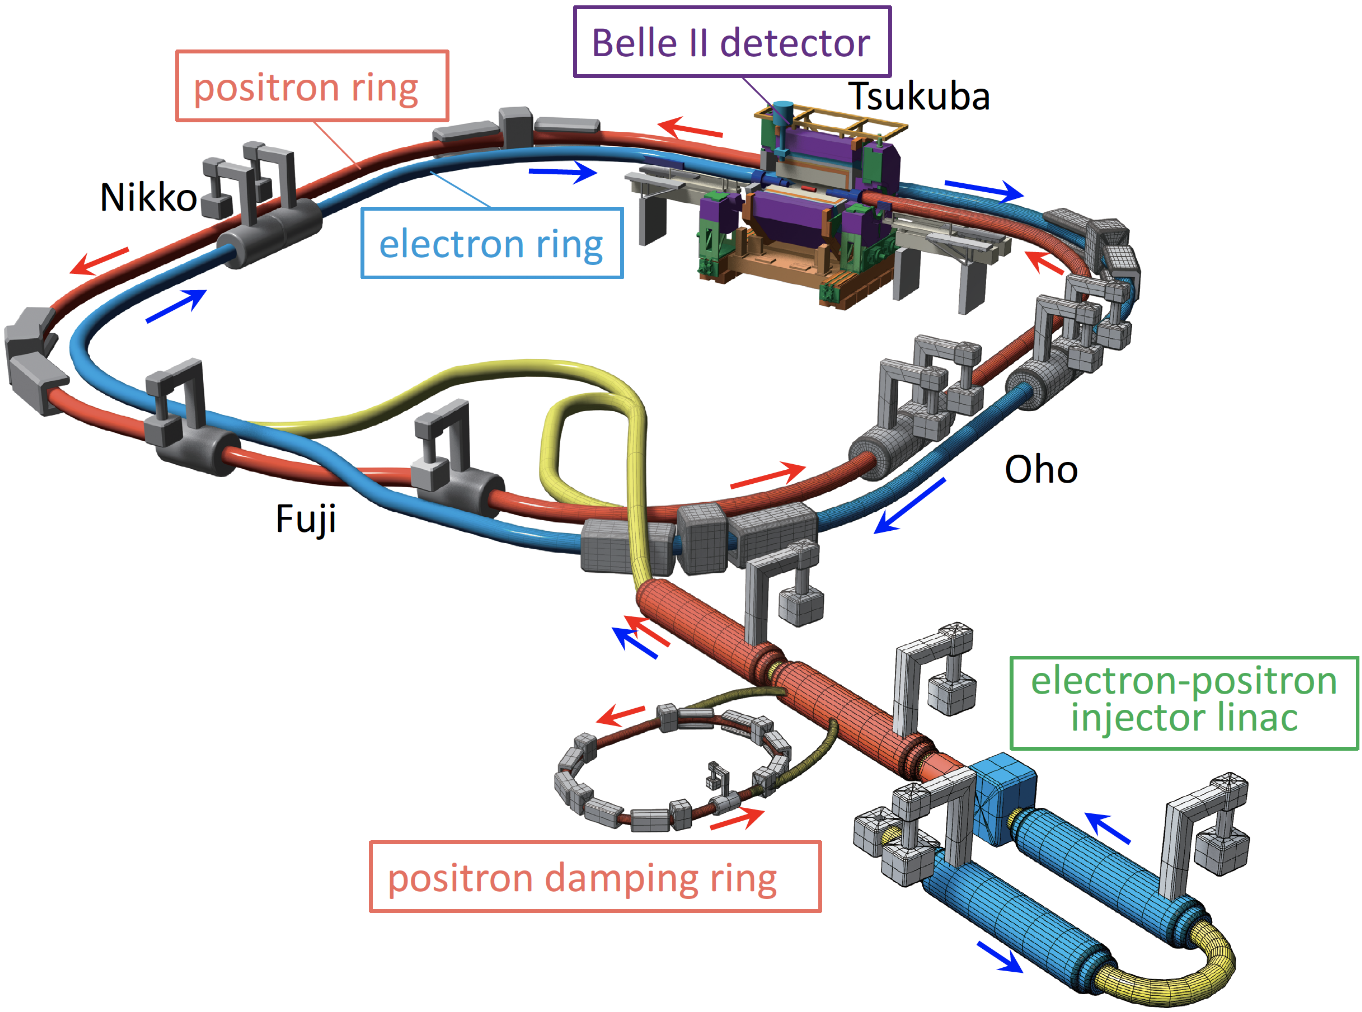
\includegraphics[width=0.6\textwidth]{figures/experimental_setup/super_kekb.png}
    \caption{\label{fig:superkekb}
        The schematic visualisation of the SuperKEKB accelerator complex.
        The main components that contribute to the acceleration of electrons and positrons are shown.
        The four straight sections are named after Japanese cities.
        Credit to \cite{Akai:2018mbz}.
    }
\end{figure}

It is important to emphasise that an \epem collision at $10.58~\gev$ produces more than just \FourS.
In truth, many other decay products including $\epem\ra\ell^+\ell^-$ or $\epem\ra\qqbar$ proceses may occur and the production 
cross-section  of all these processes depends on $\sqrt{s}$.
This is shown for $\sqrt{s}\approx10.58~\gev$ in \Cref{fig:cross_sections}, with more details about the exact values of the cross-sections provided in \Cref{sec:appendix_major_production_cross_sections}.
\begin{figure}[htbp!]
    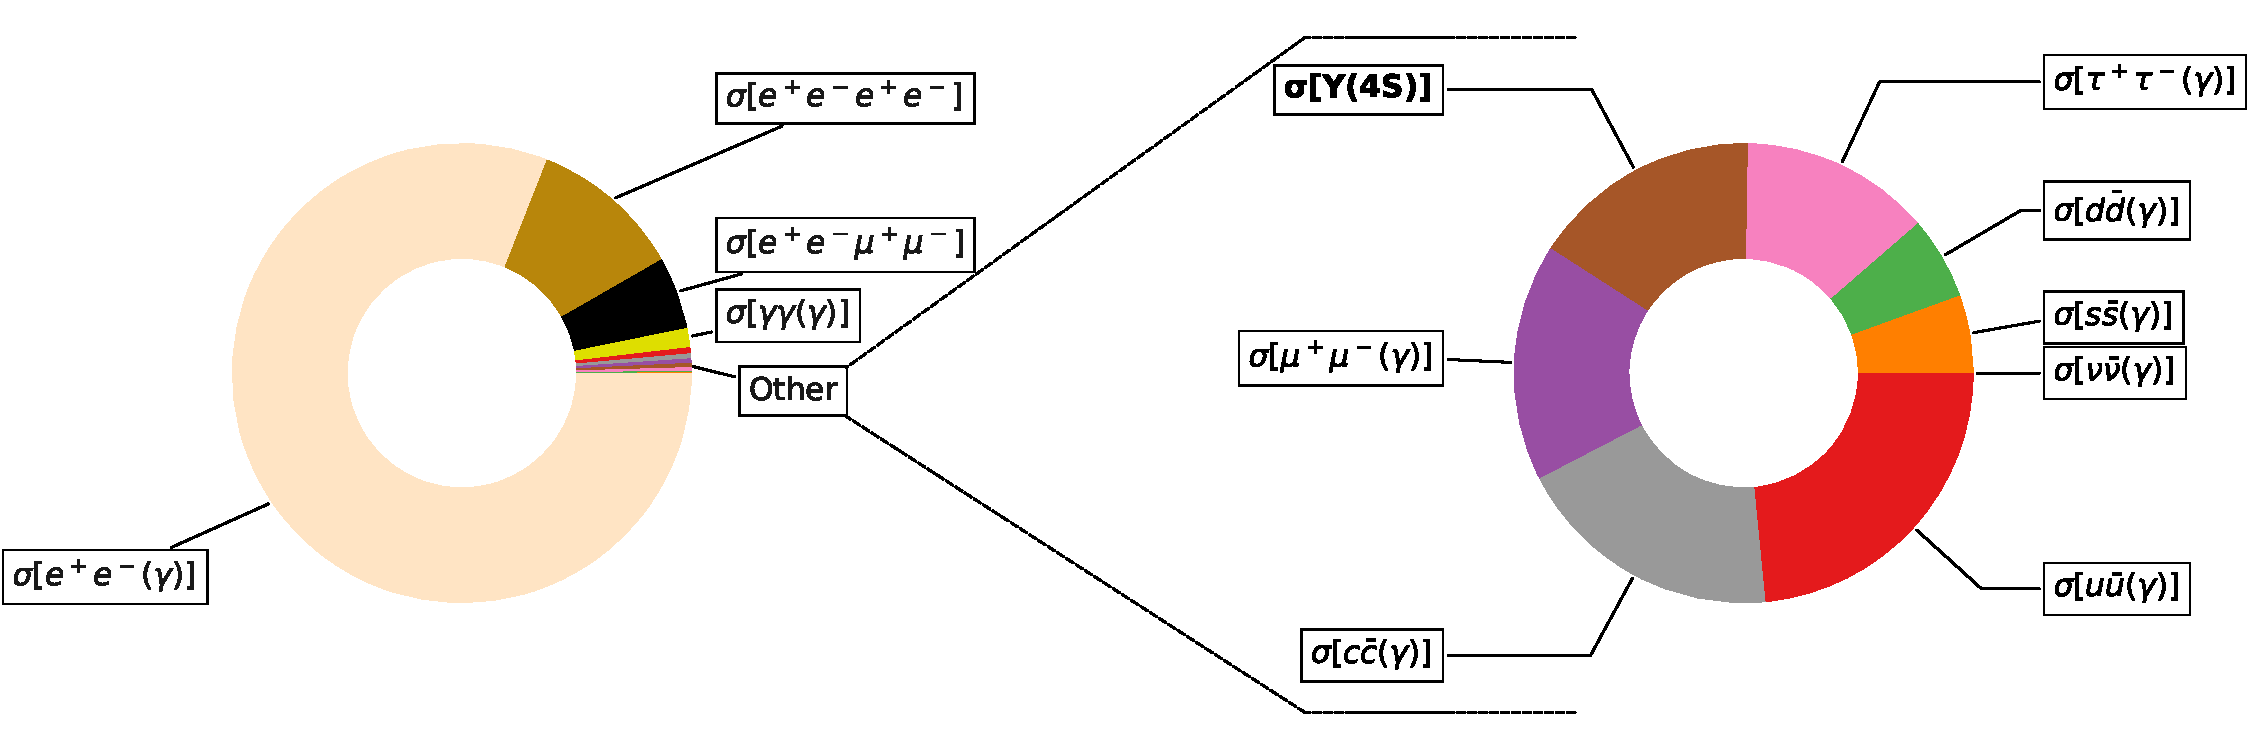
\includegraphics[width=1\textwidth]{figures/experimental_setup/corss_sections.pdf}
    \caption{\label{fig:cross_sections} Relative comparison of the largest $\epem\ra\ X$ production cross sections at $B$~factories.
    The numbers composing the charts are listed in \Cref{sec:appendix_major_production_cross_sections} and taken from \cite{Belle-II:2018jsg}.
    }
\end{figure}

Although by far the largest cross-section are related to the so-called low-multiplicity processes 
(such as $\epem\ra\epem$ and $\epem\ra\mumu$, see \Cref{sec:appendix_major_production_cross_sections}),
they differ largely from typical \FourS\ra\BB events.
On the other hand, the continuum processes (\epem\ra\qqbar ($q\in\{u,d,c,st\}$) and \epem\ra\tautau) 
events are a significant background process for many analyses aiming to measure \B meson decays
\footnote[1]{Because of the large $\epem\ra\qqbar$ and $\epem\ra\tautau$ production cross-sections, 
$B$ factories are also used to study $\tau\pm$ or $D$ meson and similar decays.
In such cases the continuum events may, in fact, be events of interest.}.

The beam-energy asymmetry (7~\gev for \en and 4~\gev for \ep) is an important design characteristic of SuperKEKB, 
which allows to separate $B$ meson vertices, necessary for measurements such as time-dependent CP violation \cite{BaBar:2014omp}.
On the other hand, the exact collision energy is chosen in order to operate at $\sqrt{(7+4)^2-(7-4)^2}\approx10.58~\gev\approx m(\FourS)$, 
hence fulfilling the requirements of the $B$~factory experiment.
The machine may also run at a 60~\mev lower collision energy, in which case $\epem\ra\FourS$ events cannot be produced.
Such data, containing only low-multiplicity and continuum events is called \textit{off-resonance} data.
Conversely, the conventional aforementioned setup is referred to as \textit{on-resonance} data.

\section{The Belle II experiment}\label{sec:belle2}

The Belle II detector, discussed in detail in Ref. \cite{Belle-II:2010dht}, is designed to reconstruct the final states of electron-positron 
collisions at center-of-mass energies at or near the \FourS meson mass.
The colliding beams are supplied by the SuperKEKB accelerator as discussed in \Cref{sec:superkekb}.

The Belle~II operates since 2018 and as of start of 2023 has collected 364~\invfb of on-resonance and 42~\invfb of off-resonance data.
The final goal is to reach 50~\invab, which will be nearly 50 times that of the combined datasets of all $B$ factories so far.

Belle II consists of several detector subsystems arranged cylindrically around the beam pipe. 
\Cref{sec:pxd} introduce the Belle~II subsystems.
The visual representation of the detector is given in \Cref{fig:belle2_detector} and shows the components of the detector, as well as their acronyms.
\begin{figure}[htbp!]
    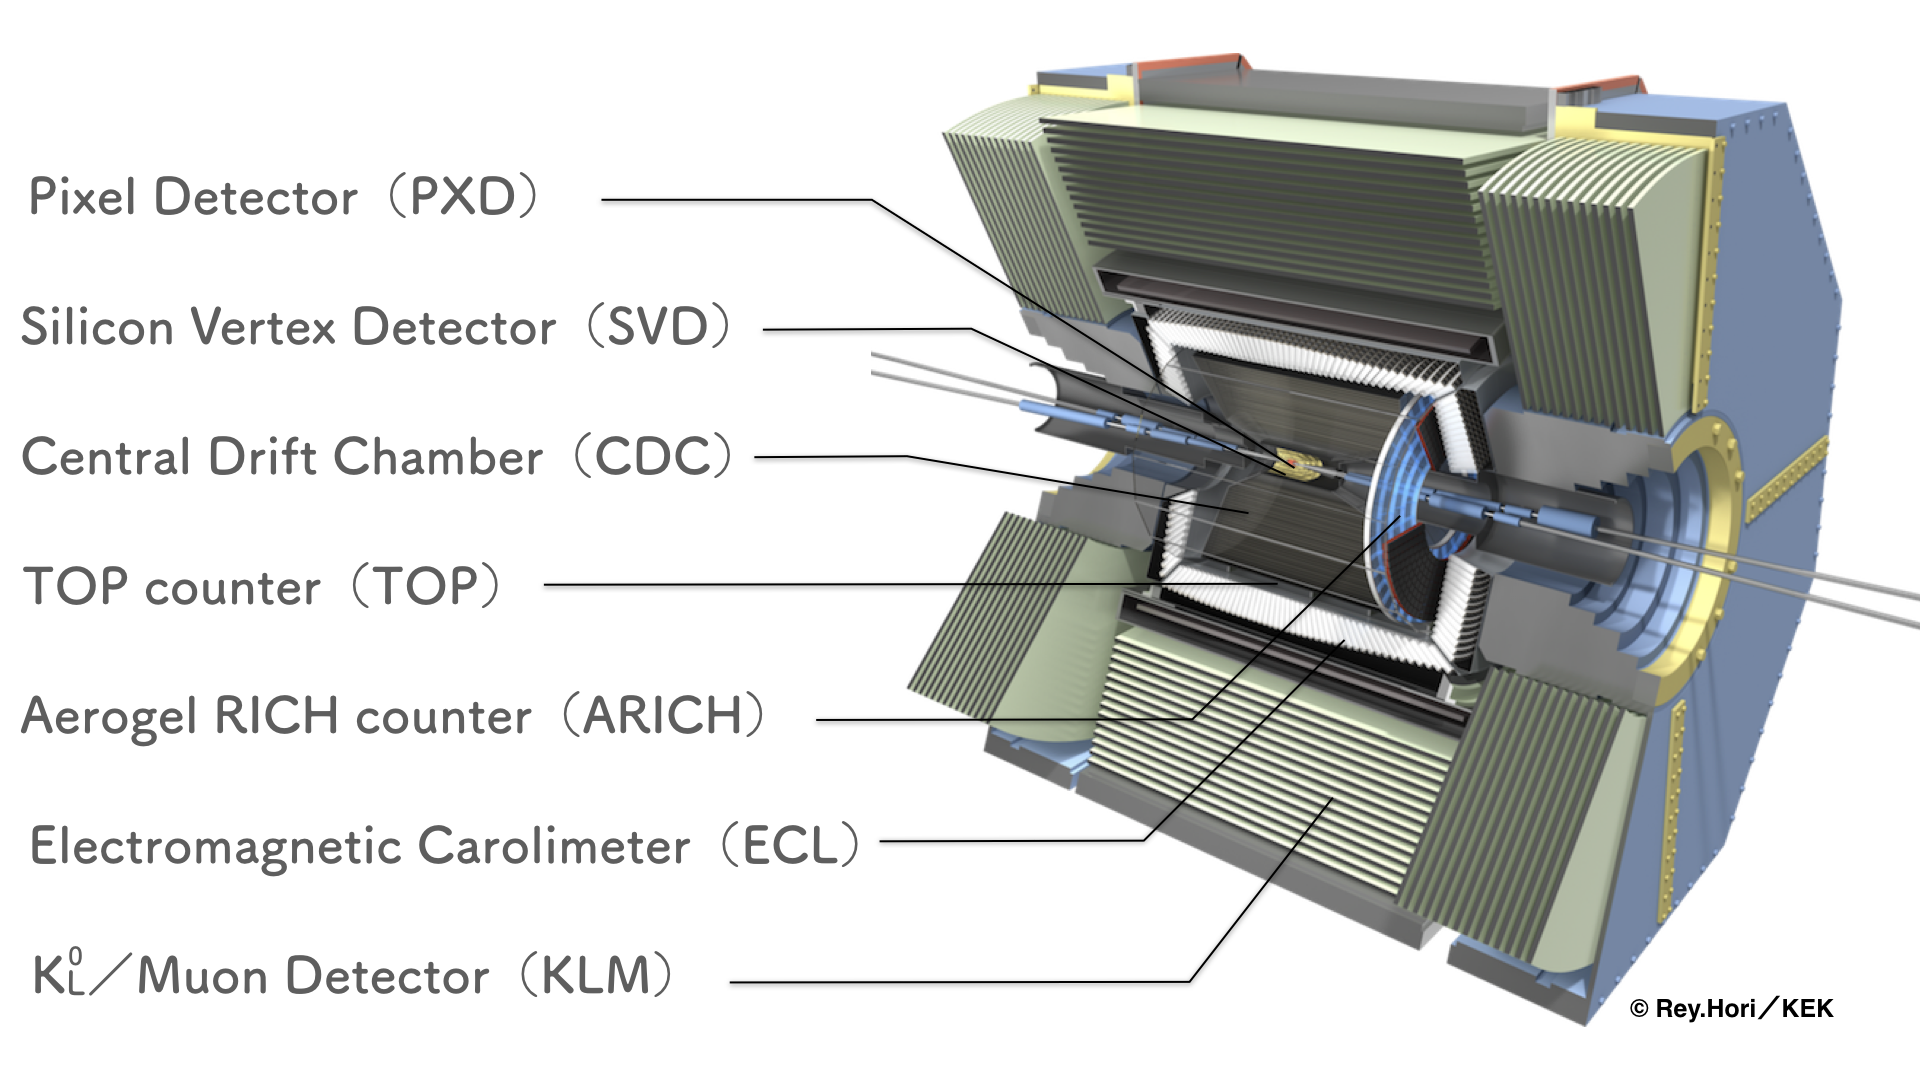
\includegraphics[width=1\textwidth]{figures/experimental_setup/belle2.png}
    \caption{\label{fig:belle2_detector} The schematic representation of the Belle~II detector.
    The Belle~II cylinder is approximately 7 meters in diameter and 7.5 meters long.
    The description of all sub systems is provided in \Cref{sec:pxd,sec:svd,sec:cdc,sec:pid,sec:magnet,sec:ecl,sec:klm}.
    Figure taken from \cite{belle_2_picture}.
    Credit to the Belle~II collaboration.
    }
\end{figure}

Belle II coordinate system is defined as follows: the $x$ axis is defined to be horizontal and points to the outside of the tunnel with respect to the accelerator's
main rings, the $y$ axis is vertically upward, and the $z$ axis is defined in the direction of the electron beam. 
The azimuthal angle, $\phi$, and the polar angle, $\theta$, are defined with respect to the $z$ axis. 
Three regions in the detector are defined based on $\theta$: 
\begin{itemize}
    \item forward endcap (\mbox{$12^{\circ}<\theta<31^{\circ}$}), 
    \item barrel (\mbox{$32^{\circ}<\theta<129^{\circ}$}),
    \item backward endcap (\mbox{$131^{\circ}<\theta<155^{\circ}$}).
\end{itemize}


\subsection{Pixel detector}\label{sec:pxd}

Closest to the collision point is the Belle~II Pixel Detector (\PXD) \cite{Belle-II:2010dht}.
Its main purpose is the high-precision detection of short-lived particle decay vertices, such as $B$ mesons.

\PXD contains two layers that use depleted $p$-channel field-effect transistors (\DEPFET) to detect charged particles that pass through it \cite{Kemmer:1986vh}.
The first layer is situated at a 14~\mm radius from the collision point, whereas the second at 22~\mm.
By design, each layer consists of 16 and 24 sensor modules, which which are glued in pairs to make 8 and 12 ladders
\footnote[1]{Until the scheduled 2023 Belle~II upgrade the outer layer contains only 2 ladders.}, respectively.
Each module contains $768\times250$ \DEPFET pixels.

The \PXD is designed to operate in large radiation conditions which it is subjected to due to the proximity to the collision point,
while maintaining high precision vertex reconstruction and a low material budget.
As a result, the sensors are able to withstand a $20~M\rad$ 
radiation dose and have a $\sim 0.2\%$ radiation length per layer \cite{Belle-II:2010dht},
while maintaining an average spatial resolution of approximately $15~\mu m$ and a hit efficiency of 99\% percent after 4 years of data taking \cite{Belle-IIDEPFET:2022wis} .
The detector is shown in \Cref{fig:pxd}, whereas its schematic location in the Belle~II detector are shown in \Cref{fig:vxd}.

\begin{figure}[htbp!]
    \centering
    \subcaptionbox{\label{fig:pxd}}{
        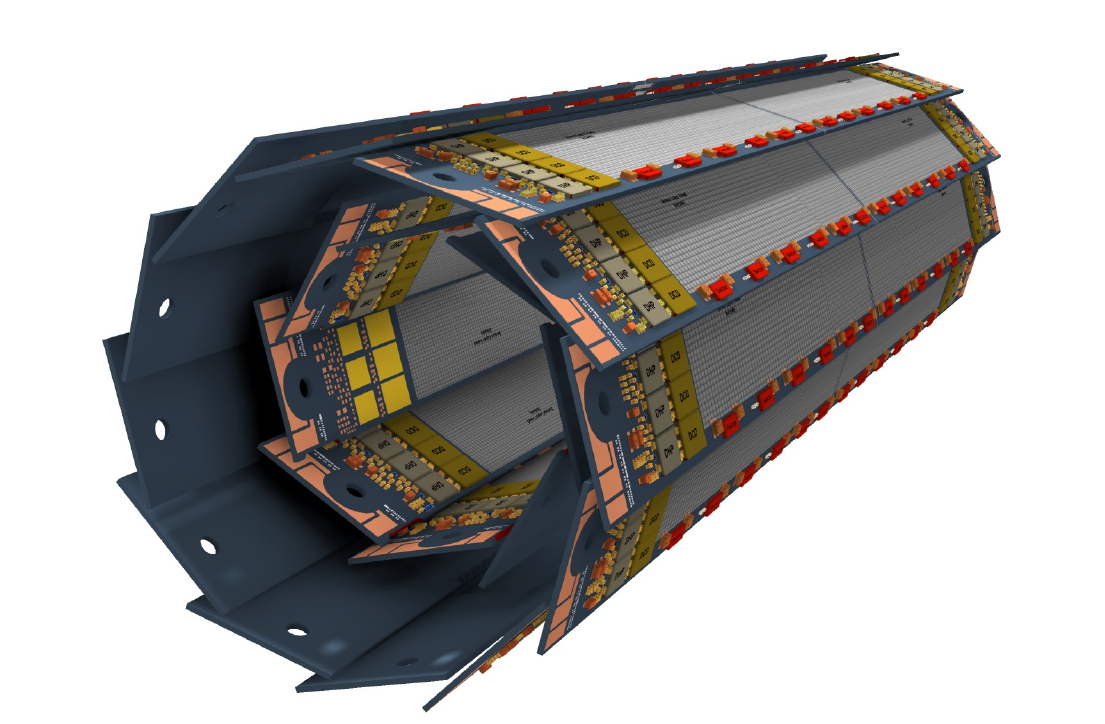
\includegraphics[width=0.45\textwidth]{figures/experimental_setup/pxd.png}
    }
    \subcaptionbox{\label{fig:svd}}{
        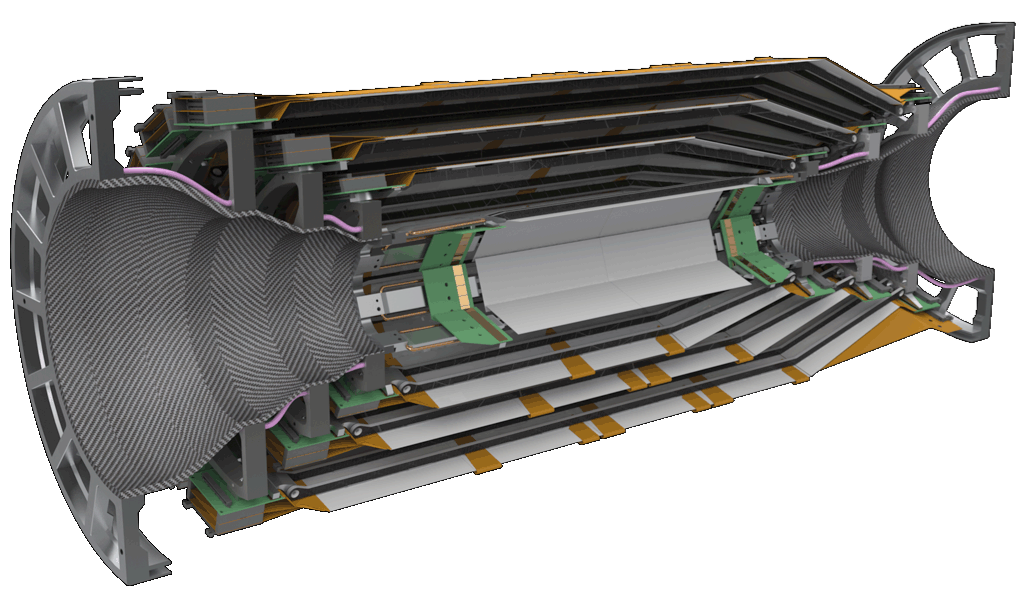
\includegraphics[width=0.45\textwidth]{figures/experimental_setup/svd.png}
    }
    \caption{\label{fig:pxd_svd} 
    The Belle II pixel detector \Cref{fig:pxd} and silicon vertex detector \Cref{fig:svd}.
    They are installed in the Belle~II detector as shown in \Cref{fig:vxd}.
    The \PXD is arranged into two layers that are designed to contain 16 modules in the first layer and 24 in the second.
    Each two layers are glued into a ladder.
    The \SVD is composed of four layers around the \PXD, with a total of 172 double-sided silicon strip sensors.
    Credit to Belle~II PXD and SVD groups.}
\end{figure}

\subsection{Silicon vertex detector}\label{sec:svd}

The silicon vertex detector (\SVD) \cite{Belle-IISVD:2023mxk} surrounds the \PXD and 
is the second subsystem responsible for charged particle detection.
Its main roles include the reconstruction of short-lived particle decay vertices in conjunction with PXD,
standalone charged particle trajectory reconstruction (for low momentum particles),
and particle identification information through specific ionisiation measurements.

The \SVD contains four layers. 
The first layer is composed of 7 ladders with 2 sensors,
the second -- of 10 ladders with 3 sensors,
the third -- of 12 ladders with 4 sensors,
and the final of 16 ladders with 5 sensors.
The 172 double-sided silicon strip sensors are composed, in total, of 224 thousand strips.
Each sensor is based on an $n$-type bulk implanted with $p$ and $n$-doped sensitive strips on opposite sides.
The schematic representation of \SVD is shown in \Cref{fig:svd}, whereas its schematic location in the Belle~II detector are shown in \Cref{fig:vxd}.

\begin{figure}[htbp!]
    \centering
    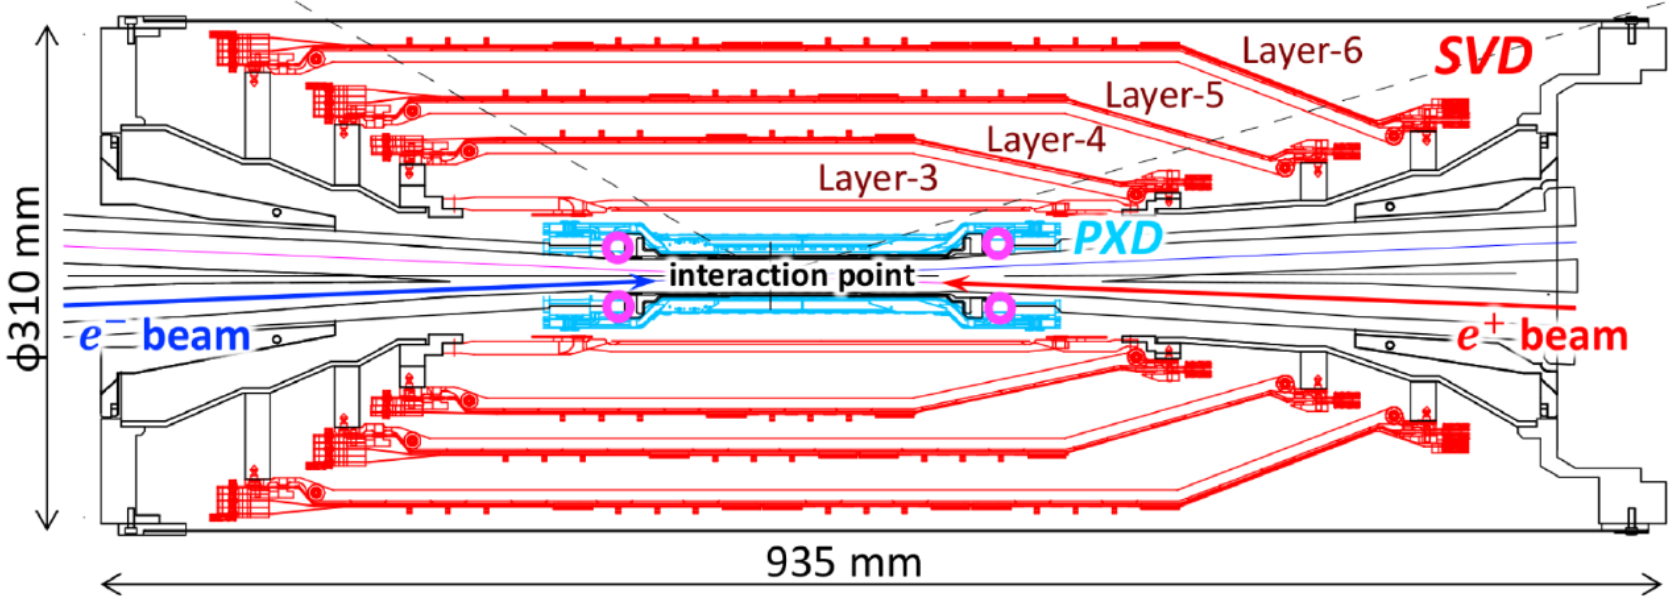
\includegraphics[width=0.6\textwidth]{figures/experimental_setup/vxd.png}
    \caption{\label{fig:vxd}
    The Belle II pixel detector and silicon vertex detector shown inside of the Belle~II detector.
    The size of the both vertex detection components, as well as the interaction point are noted.
    Credit to \cite{Belle-IISVD:2023mxk}.
    }
\end{figure}

\subsection{Central Drift Chamber}\label{sec:cdc}

The central drift chamber (\CDC) \cite{Taniguchi:2017not} is the central subsystem responsible for the reconstruction of charged particle trajectories inside the Belle~II experiment.
As such, its main objective is the detection of particle momenta and charge.
The \CDC also provides particle identification information through specific ionisation measurements
and participates in the decision to save the event information (\textit{triggering}).

It is a large volume drift chamber filled with a 50\% helium and 50\% ethane mixture.
The \CDC begins immediately after \SVD at $160~\mm$ and is contained within an outer cylinder radius of $1130~\mm$
It consists of 14336 readout wires distributed across 56 layers.
Each readout is surrounded by 8 field wires that create an electric field in the chamber.
As a charged particle passes through the chamber ionising the gas,
the electrons are accelerated in the electric field creating avalanches that are read out as signal by the wires.
In order to obtain three-dimensional information about the particle trajectory,
some layers in the \CDC are skewed.
The first 8 layers are axial, whereas the rest alternate between axial and skewed every 6 layers.
The grouping of layers is shown in \Cref{fig:cdc_quadrant}, whereas \Cref{fig:cdc_wires} illustrate the difference between axial ad skewed layers.

The \CDC provides a highly accurate measurement of charged particle trajectories with a $0.1-0.2~\cm$ spatial resolution 
and a $~\sim0.5\%$ momentum resolution for the majority of particles resulting in \B meson decays \cite{Kandra:2019qlz}.

\begin{figure}[htbp!]
    \centering
    \subcaptionbox{\label{fig:cdc_quadrant}}{
        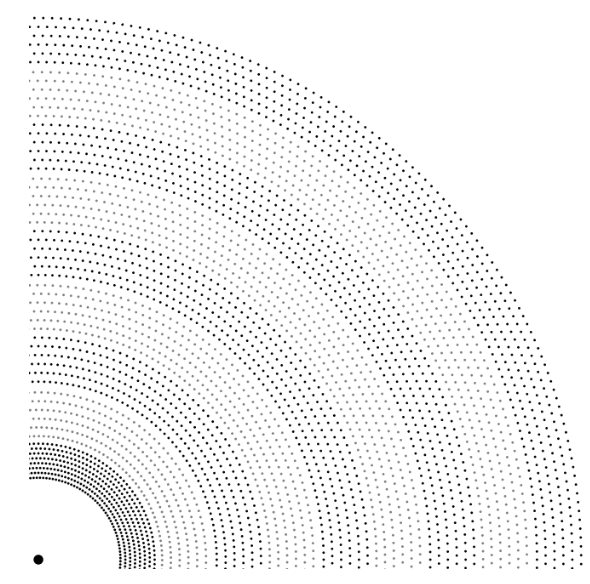
\includegraphics[width=0.45\textwidth]{figures/experimental_setup/cdc_quadrant.png}
    }
    \subcaptionbox{\label{fig:cdc_wires}}{
        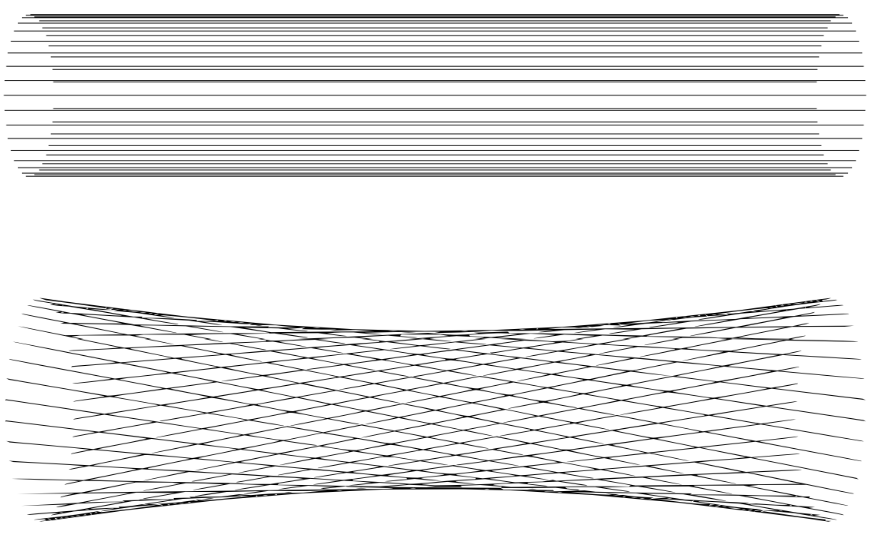
\includegraphics[width=0.45\textwidth]{figures/experimental_setup/cdc_layers.png}
    }
    \caption{\label{fig:cdc}
    The Belle~II central drift chamber schematic representation.
    \Cref{fig:cdc_quadrant} shows a quadrant of the \CDC in the $r$-$\phi$ plane.
    Different axial and skewed layer groups are visible.
    \Cref{fig:cdc_wires} show the axial (upper) and (skewed) wires.
    The skew is exaggerated for illustrative purposes.
    Credit to \cite{BelleIITrackingGroup:2020hpx}.
    }
\end{figure}

\subsection{Particle identification systems}\label{sec:pid}

\subsection{Electromagnetinc Calorimeter}\label{sec:ecl}

\subsection{Magnet}\label{sec:magnet}

\subsection{\texorpdfstring{$K_L$}{KL} and \texorpdfstring{\mu}{mu} detector}\label{sec:klm}



